When discussing the drawbacks of such a system, many problems may arise during the installation, usage and maintenance process. Here are a few examples that our team has brainstormed:
\begin{enumerate}
    \item Scalability
\end{enumerate}
In the study above, Emma Zhang and Luping Tang used coated-metal electrodes with a dimension of 100 mm $\times$ 100 mm $\times$ 4 mm, while the dimension of the metal-coated CF meshes was 90 mm $\times$ 90 mm $\times$ 1 mm. 

\begin{enumerate}[resume]
    \item Difficulty to install in vertical walls
\end{enumerate}
The diagram below illustrates the method the researchers used to construct their model:
\begin{figure}[H]
\centering
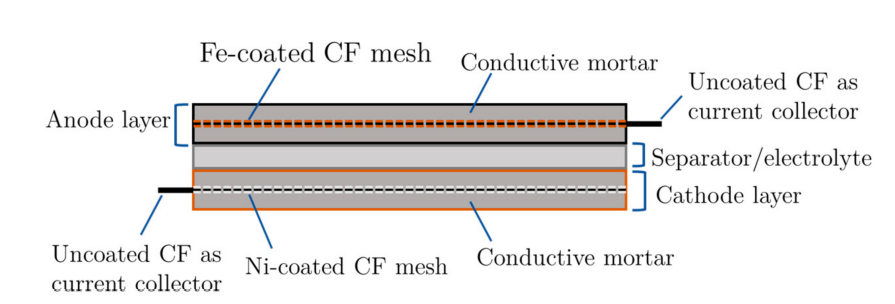
\includegraphics[scale=0.75]{A}
\caption{The 'sandwich' model utilised in cement batteries}
\label{fig:bat}
\end{figure}
The researchers had to embed the metal-coated CF mesh within the cement for the battery to function. When pouring the cement into the cast, the cement had to be spreaded out into thin layers so that the results would be consistent. However, during the construction of a vertical wall, each concrete brick will be laid out alternatingly with steel beams, before grout concrete is poured between the spaces to strengthen the wall.
\begin{figure}[H]
\centering
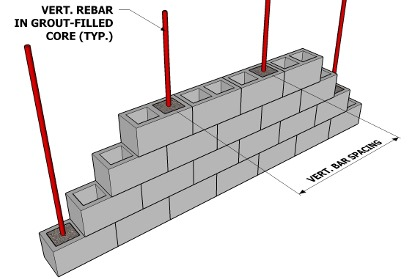
\includegraphics[scale=0.75]{B}
\caption{Construction of concrete walls}\cite{theconstructor:walls}
\end{figure}
This will lead to difficulties during both the construction of walls and installation of cement batteries, which have not been solved yet.

\begin{enumerate}[resume]
    \item Maintenance issues
\end{enumerate}
As concrete walls are constructed using the above method, it will be impossible to investigate issues that may arise during the maintenance process without harming the internal structures of the building. Because the insides of a wall is solid, parts of the wall will have to be destroyed and rebuilt in order to fix issues. Consequently, the maintenance process will be costly and potentially be disruptive to both the electric grid and the family.